\documentclass[aspectratio=169]{beamer}

% ============================================
% PACOTES ADICIONAIS
% ============================================
\usepackage[utf8]{inputenc}
\usepackage[T1]{fontenc}
\usepackage{amsmath}
\usepackage{amsfonts}
\usepackage{amssymb}
\usepackage{graphicx}
\usepackage{hyperref}
\usepackage{ifthen}
\usepackage{bm}
\usepackage{array}
\usepackage{tikz}
\usetikzlibrary{shapes.geometric, arrows.meta, positioning, decorations.pathreplacing,
                calc, fit, backgrounds, shadows}
\usepackage{listings}

% ============================================
% CONFIGURACAO DO LISTINGS (código)
% ============================================
\definecolor{codebg}{RGB}{245,245,245}
\definecolor{codegreen}{RGB}{0,128,0}
\definecolor{codegray}{RGB}{128,128,128}
\definecolor{codeblue}{RGB}{0,0,180}

\lstset{
  basicstyle=\ttfamily\tiny,
  backgroundcolor=\color{codebg},
  keywordstyle=\color{codeblue}\bfseries,
  commentstyle=\color{codegreen},
  stringstyle=\color{red!60!black},
  showstringspaces=false,
  frame=single,
  rulecolor=\color{gray!40},
  breaklines=true,
  columns=fullflexible,
}

% ============================================
% VARIAVEIS DE CONFIGURACAO
% ============================================
\newcommand{\autorNome}{Prof. Daniel Costa Araujo}
\newcommand{\autorEmail}{daniel.araujo@unb.br}
\newcommand{\tituloApresentacao}{Laborat\'{o}rio PRICOM}
\newcommand{\subtituloApresentacao}{Introduc\~{a}o ao GNU Radio --- Primeiros Passos}
\newcommand{\idioma}{pt}
\newcommand{\universidadePT}{Universidade de Brasilia}
\newcommand{\departamentoPT}{Faculdade de Ciencias e Tecnologia em Engenharias}
\newcommand{\laboratorioPT}{Laboratorio de Telecomunicacoes}
\newcommand{\universidadeEN}{University of Brasilia}
\newcommand{\departamentoEN}{Faculty of Sciences and Technology in Engineering}
\newcommand{\laboratorioEN}{Telecommunications Laboratory}
\newcommand{\dataApresentacao}{2026}

\newcommand{\institutoFinal}{%
    \ifthenelse{\equal{\idioma}{pt}}{\universidadePT \\ \laboratorioPT}%
                                    {\universidadeEN \\ \laboratorioEN}%
}
\newcommand{\universidadeFinal}{%
    \ifthenelse{\equal{\idioma}{pt}}{\universidadePT}{\universidadeEN}%
}
\newcommand{\laboratorioFinal}{%
    \ifthenelse{\equal{\idioma}{pt}}{\laboratorioPT}{\laboratorioEN}%
}

% ============================================
\definecolor{unbprimary}{RGB}{0,59,92}
\colorlet{cOrange}{orange!80!black}
\colorlet{cBlue}{blue!70!black}
\colorlet{cTeal}{teal!70!black}
\colorlet{cRed}{red!60!black}
\colorlet{cPurple}{purple!70!black}
\colorlet{cGreen}{green!50!black}
% CARREGAR TEMPLATE UnB/LabTelecom
% ============================================
\graphicspath{{../../../figures_global/}}
% Template Beamer para UnB/LabTelecom
% Cores da UnB
\definecolor{unbprimary}{RGB}{0,59,92}      % #003B5C
\definecolor{unbsecondary}{RGB}{0,102,51}   % #006633
\definecolor{unbaccent}{RGB}{242,169,0}      % #F2A900


% Configuração do tema
\usetheme{Madrid}
\usecolortheme{default}

% Aplicar cores UnB
\setbeamercolor{structure}{fg=unbprimary}
\setbeamercolor{title}{fg=white}
\setbeamercolor{frametitle}{fg=white}
\setbeamercolor{section in toc}{fg=unbprimary}
\setbeamercolor{subsection in toc}{fg=unbsecondary}

% Configurações de fonte
\setbeamerfont{title}{size=\huge,series=\bfseries}
\setbeamerfont{frametitle}{size=\Large,series=\bfseries}



% Cabeçalho com logos
\setbeamertemplate{headline}{
  \begin{beamercolorbox}[wd=\paperwidth,ht=1.2cm]{headline}
    \hspace{0.5cm}%
    \raisebox{0.2cm}{
\includegraphics[height=0.8cm]{../../figures_global/unb.png}}%
    \hfill%
    \raisebox{0.35cm}{\textcolor{unbprimary}{\textbf{\universidadeFinal}}}%
    \hfill%
    \raisebox{0.2cm}{
\includegraphics[height=0.8cm]{../../figures_global/labtelecom.png}}%
    \hspace{0.5cm}%
  \end{beamercolorbox}
}

% Rodapé
\setbeamertemplate{footline}{
  \begin{beamercolorbox}[wd=\paperwidth,ht=0.5cm]{footline}
    \hspace{1cm}
    \textcolor{unbprimary}{\insertshorttitle}
    \hfill
    \textcolor{unbprimary}{\insertframenumber/\inserttotalframenumber}
    \hspace{1cm}
  \end{beamercolorbox}
}

% Remover símbolos de navegação e mini frames (evita conflito com TikZ)
\setbeamertemplate{navigation symbols}{}
\setbeamertemplate{mini frames}{}
\setbeamertemplate{mini frame in current subsection}{}
\setbeamertemplate{mini frame in other section}[default]

% ============================================
% APLICAR CONFIGURACOES
% ============================================
\title{\tituloApresentacao}
\subtitle{\subtituloApresentacao}
\author{\autorNome}
\institute{\institutoFinal}
\date{\dataApresentacao}

% Comandos uteis
\newcommand{\figFull}{0.85\textwidth}
\newcommand{\figHalf}{0.65\textwidth}
\newcommand{\figHalfV}{0.48\textwidth}

% Estilos TikZ para blocos GRC
\tikzset{
  grcblock/.style={rectangle, rounded corners=3pt, draw=gray!60,
                   minimum width=2.0cm, minimum height=0.7cm,
                   align=center, font=\scriptsize},
  grcsrc/.style={grcblock, fill=green!20},
  grcproc/.style={grcblock, fill=blue!15},
  grcsink/.style={grcblock, fill=red!20},
  grcvar/.style={grcblock, fill=yellow!20, draw=orange!60},
  grcthrottle/.style={grcblock, fill=purple!15, draw=purple!40},
  grcarrow/.style={->, thick, gray!70},
}

% ============================================
\begin{document}

% --- TITULO ---
\begin{frame}
\titlepage
\end{frame}

% --- SUMARIO ---
\begin{frame}{Sum\'{a}rio}
\small
\tableofcontents[hideallsubsections]
\end{frame}

% %%%%%%%%%%%%%%%%%%%%%%%%%%%%%%%%%%%%%%%%%%%%
\section{O que \'{e} o GNU Radio?}
% %%%%%%%%%%%%%%%%%%%%%%%%%%%%%%%%%%%%%%%%%%%%

{
\setbeamercolor{background canvas}{bg=unbprimary}
\setbeamercolor{normal text}{fg=white}
\usebeamercolor[fg]{normal text}
\begin{frame}[plain,c]
\begin{center}
{\Huge\textbf{O que \'{e} o GNU Radio?}}\\[0.8cm]
{\LARGE Ferramenta open-source para SDR}\\[0.5cm]
{\large Processamento de sinais com blocos gr\'{a}ficos}
\end{center}
\end{frame}
}

% --- Slide GRC comentado ---
\iffalse
\begin{frame}{GNU Radio Companion (GRC)}
\begin{center}
  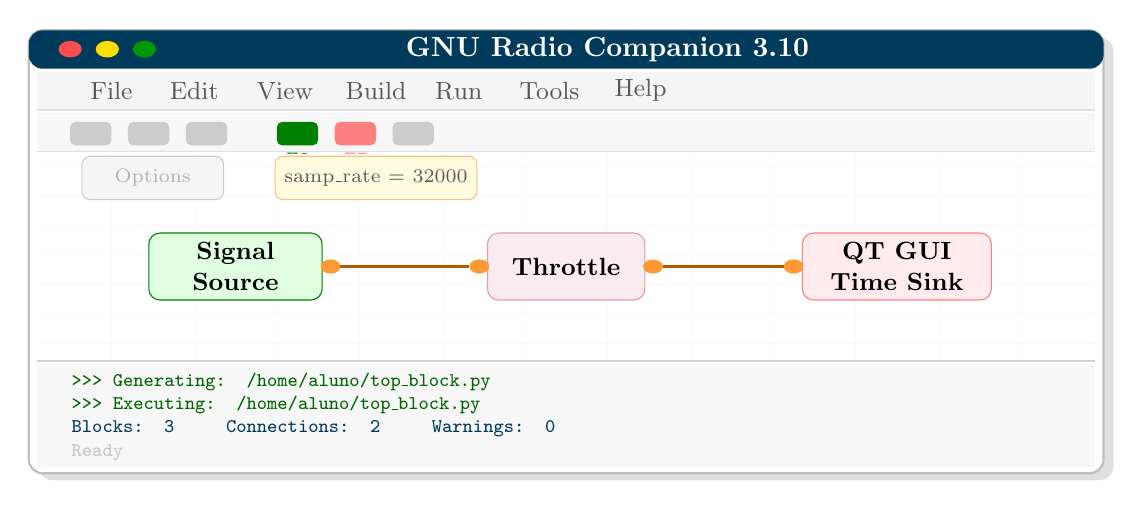
\begin{tikzpicture}[xscale=1.05, yscale=0.75]
    % --- Sombra da janela ---
    \fill[black!12, rounded corners=5pt] (0.12,-0.12) rectangle (13.12, 7.38);
    % --- Janela principal ---
    \draw[rounded corners=5pt, thick, gray!50, fill=white]
      (0,0) rectangle (13.0, 7.5);
    % --- Barra de titulo ---
    \fill[unbprimary, rounded corners=5pt]
      (0,6.85) -- (13.0,6.85) -- (13.0,7.5) -- (0,7.5) -- cycle;
    \fill[red!70] (0.5, 7.18) circle (0.14);
    \fill[yellow!80!orange] (0.95, 7.18) circle (0.14);
    \fill[green!60!black] (1.4, 7.18) circle (0.14);
    \node[text=white, font=\normalsize\bfseries] at (7.0,7.18) {GNU Radio Companion 3.10};
    % --- Menu bar ---
    \fill[gray!8] (0.1,6.15) rectangle (12.9,6.8);
    \draw[gray!25] (0.1,6.15) -- (12.9,6.15);
    \node[font=\small, text=gray!70!black] at (1.0,6.48) {File};
    \node[font=\small, text=gray!70!black] at (2.0,6.48) {Edit};
    \node[font=\small, text=gray!70!black] at (3.1,6.48) {View};
    \node[font=\small, text=gray!70!black] at (4.2,6.48) {Build};
    \node[font=\small, text=gray!70!black] at (5.2,6.48) {Run};
    \node[font=\small, text=gray!70!black] at (6.3,6.48) {Tools};
    \node[font=\small, text=gray!70!black] at (7.4,6.48) {Help};
    % --- Toolbar icons ---
    \fill[gray!6] (0.1,5.45) rectangle (12.9,6.1);
    \draw[gray!25] (0.1,5.45) -- (12.9,5.45);
    \foreach \x/\c in {0.5/gray!40, 1.2/gray!40, 1.9/gray!40, 3.0/green!50!black, 3.7/red!50, 4.4/gray!40} {
      \fill[\c, rounded corners=2pt] (\x, 5.55) rectangle ({\x+0.5}, 5.95);
    }
    \node[font=\tiny\bfseries, text=green!50!black] at (3.25, 5.35) {F6};
    \node[font=\tiny\bfseries, text=red!50] at (3.95, 5.35) {F7};
    % --- Canvas ---
    \fill[white] (0.1,1.9) rectangle (12.9,5.4);
    \foreach \x in {1,2,...,12} { \draw[gray!6] (\x,1.9) -- (\x,5.4); }
    \foreach \y in {2.2,2.7,...,5.2} { \draw[gray!6] (0.1,\y) -- (12.9,\y); }
    % --- Blocos do topo ---
    \node[rectangle, rounded corners=3pt, draw=gray!40, fill=gray!8,
          minimum width=1.8cm, minimum height=0.55cm,
          font=\scriptsize, text=gray!60] at (1.5, 5.0) {Options};
    \node[rectangle, rounded corners=3pt, draw=orange!50, fill=yellow!12,
          minimum width=2.2cm, minimum height=0.55cm,
          font=\scriptsize, text=gray!70!black] at (4.2, 5.0) {samp\_rate = 32000};
    % --- Flowgraph ---
    \node[rectangle, rounded corners=4pt, draw=green!50!black, fill=green!12,
          minimum width=2.2cm, minimum height=0.85cm,
          font=\small\bfseries, align=center] (src) at (2.5, 3.5) {Signal\\Source};
    \fill[orange!80] (3.65, 3.5) circle (0.12);
    %
    \node[rectangle, rounded corners=4pt, draw=purple!40, fill=purple!8,
          minimum width=2.0cm, minimum height=0.85cm,
          font=\small\bfseries, align=center] (thr) at (6.5, 3.5) {Throttle};
    \fill[orange!80] (5.45, 3.5) circle (0.12);
    \fill[orange!80] (7.55, 3.5) circle (0.12);
    %
    \node[rectangle, rounded corners=4pt, draw=red!50, fill=red!8,
          minimum width=2.4cm, minimum height=0.85cm,
          font=\small\bfseries, align=center] (snk) at (10.5, 3.5) {QT GUI\\Time Sink};
    \fill[orange!80] (9.25, 3.5) circle (0.12);
    % Conexoes
    \draw[very thick, orange!70!black] (3.77, 3.5) -- (5.33, 3.5);
    \draw[very thick, orange!70!black] (7.67, 3.5) -- (9.13, 3.5);
    % --- Divisor canvas/console ---
    \draw[gray!35, thick] (0.1,1.9) -- (12.9,1.9);
    % --- Console ---
    \fill[gray!6] (0.1,0.1) rectangle (12.9,1.85);
    \node[anchor=west, font=\scriptsize\ttfamily, text=green!40!black] at (0.4,1.55)
      {>>> Generating: /home/aluno/top\_block.py};
    \node[anchor=west, font=\scriptsize\ttfamily, text=green!40!black] at (0.4,1.15)
      {>>> Executing: /home/aluno/top\_block.py};
    \node[anchor=west, font=\scriptsize\ttfamily, text=unbprimary] at (0.4,0.75)
      {Blocks: 3 \quad\quad Connections: 2 \quad\quad Warnings: 0};
    \node[anchor=west, font=\scriptsize\ttfamily, text=gray!45] at (0.4,0.35)
      {Ready};
  \end{tikzpicture}
\end{center}
\end{frame}
\fi

\begin{frame}{O que \'{e} o GNU Radio?}
\begin{itemize}\setlength{\itemsep}{3pt}
  \item Plataforma \textbf{open-source} para processamento de sinais
  \item Interface gr\'{a}fica: \textbf{GNU Radio Companion (GRC)}
  \item Programa\c{c}\~{a}o visual: \textbf{blocos} conectados por \textbf{fluxos} de dados
  \item Gera c\'{o}digo \textbf{Python} automaticamente a partir do diagrama
  \item Usado em pesquisa, ensino e ind\'{u}stria (SDR)
\end{itemize}
\end{frame}

\begin{frame}{Conceito fundamental: \textit{flowgraph}}
\begin{center}
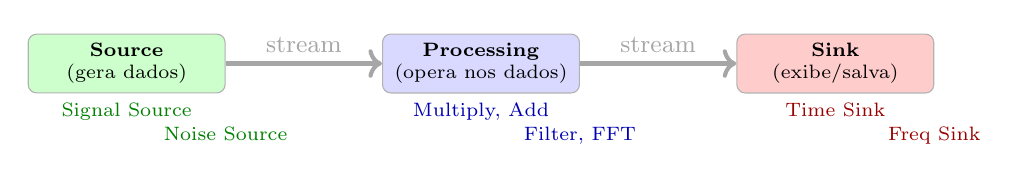
\begin{tikzpicture}[scale=1.0]
  % Fonte
  \node[grcsrc, minimum width=2.5cm] (src) at (0,0) {\textbf{Source}\\(gera dados)};
  % Processamento
  \node[grcproc, minimum width=2.5cm] (proc) at (4.5,0) {\textbf{Processing}\\(opera nos dados)};
  % Sink
  \node[grcsink, minimum width=2.5cm] (sink) at (9,0) {\textbf{Sink}\\(exibe/salva)};
  % Setas
  \draw[grcarrow, line width=1.5pt] (src) -- node[above, font=\small] {stream} (proc);
  \draw[grcarrow, line width=1.5pt] (proc) -- node[above, font=\small] {stream} (sink);
  % Labels
  \node[below, font=\scriptsize, text=cGreen] at (src.south) {Signal Source};
  \node[below, font=\scriptsize, text=cGreen] at (src.south east) [yshift=-0.3cm] {Noise Source};
  \node[below, font=\scriptsize, text=cBlue] at (proc.south) {Multiply, Add};
  \node[below, font=\scriptsize, text=cBlue] at (proc.south east) [yshift=-0.3cm] {Filter, FFT};
  \node[below, font=\scriptsize, text=cRed] at (sink.south) {Time Sink};
  \node[below, font=\scriptsize, text=cRed] at (sink.south east) [yshift=-0.3cm] {Freq Sink};
\end{tikzpicture}
\end{center}

\vspace{0.3cm}

\begin{columns}
\begin{column}{0.48\textwidth}
  \textbf{Estrutura b\'{a}sica:}
  \begin{enumerate}
    \item \textbf{Source}: gera ou recebe o sinal
    \item \textbf{Processing}: opera matematicamente
    \item \textbf{Sink}: exibe, grava ou transmite
  \end{enumerate}
\end{column}
\begin{column}{0.48\textwidth}
  \textbf{Regras do fluxo:}
  \begin{itemize}
    \item Dados fluem da \textbf{esquerda para a direita}
    \item Portas devem ter \alert{mesmo tipo de dado}
    \item Cores das portas indicam o tipo
  \end{itemize}
\end{column}
\end{columns}
\end{frame}

% %%%%%%%%%%%%%%%%%%%%%%%%%%%%%%%%%%%%%%%%%%%%
\section{Tipos de Dados no GNU Radio}
% %%%%%%%%%%%%%%%%%%%%%%%%%%%%%%%%%%%%%%%%%%%%

{
\setbeamercolor{background canvas}{bg=unbprimary}
\setbeamercolor{normal text}{fg=white}
\usebeamercolor[fg]{normal text}
\begin{frame}[plain,c]
\begin{center}
{\Huge\textbf{Tipos de Dados}}\\[0.8cm]
{\LARGE As cores das portas dos blocos}\\[0.5cm]
{\large Complex, Float, Int, Short, Byte}
\end{center}
\end{frame}
}

\begin{frame}{Tipos de dados e cores das portas}
\begin{columns}
\begin{column}{0.55\textwidth}
  \textbf{Cada porta tem um tipo e uma cor:}

  \vspace{0.15cm}

  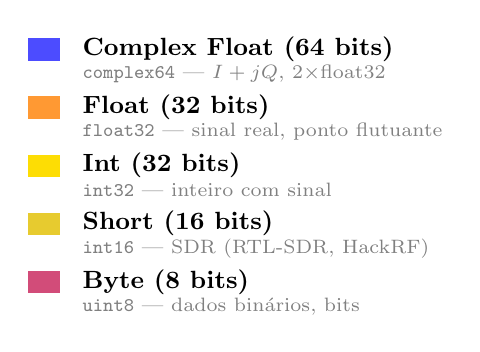
\begin{tikzpicture}[scale=0.82]
    % Complex Float (azul)
    \fill[blue!70] (0, 3.6) rectangle (0.5, 3.95);
    \node[right, font=\small\bfseries] at (0.7, 3.78) {Complex Float (64 bits)};
    \node[right, font=\scriptsize, text=gray] at (0.7, 3.4) {\texttt{complex64} --- $I + jQ$, 2$\times$float32};

    % Float (laranja)
    \fill[orange!80] (0, 2.7) rectangle (0.5, 3.05);
    \node[right, font=\small\bfseries] at (0.7, 2.88) {Float (32 bits)};
    \node[right, font=\scriptsize, text=gray] at (0.7, 2.5) {\texttt{float32} --- sinal real, ponto flutuante};

    % Int (amarelo)
    \fill[yellow!80!orange] (0, 1.8) rectangle (0.5, 2.15);
    \node[right, font=\small\bfseries] at (0.7, 1.98) {Int (32 bits)};
    \node[right, font=\scriptsize, text=gray] at (0.7, 1.6) {\texttt{int32} --- inteiro com sinal};

    % Short (amarelo escuro)
    \fill[yellow!60!brown] (0, 0.9) rectangle (0.5, 1.25);
    \node[right, font=\small\bfseries] at (0.7, 1.08) {Short (16 bits)};
    \node[right, font=\scriptsize, text=gray] at (0.7, 0.7) {\texttt{int16} --- SDR (RTL-SDR, HackRF)};

    % Byte (roxo)
    \fill[purple!70] (0, 0.0) rectangle (0.5, 0.35);
    \node[right, font=\small\bfseries] at (0.7, 0.18) {Byte (8 bits)};
    \node[right, font=\scriptsize, text=gray] at (0.7, -0.2) {\texttt{uint8} --- dados bin\'{a}rios, bits};
  \end{tikzpicture}
\end{column}
\begin{column}{0.42\textwidth}
  \begin{alertblock}{Regra fundamental}
  \small Portas conectadas devem ter a \textbf{mesma cor} (mesmo tipo).\\[0.15cm]
  Se precisar converter:\\
  \texttt{Float To Complex}\\
  \texttt{Complex To Real}\\
  \texttt{Complex To Mag}
  \end{alertblock}

  \vspace{0.15cm}

  \begin{exampleblock}{Na pr\'{a}tica}
  \small \textbf{90\% do tempo} usamos:\\
  --- \textcolor{blue!70}{\textbf{Complex}} (sinais RF)\\
  --- \textcolor{orange!80}{\textbf{Float}} (sinais banda-base)
  \end{exampleblock}
\end{column}
\end{columns}
\end{frame}

\begin{frame}{Complex vs.\ Float --- quando usar cada um?}
\begin{columns}
\begin{column}{0.48\textwidth}
  \begin{block}{\textcolor{blue!70}{Complex Float} --- sinal anal\'{\i}tico}
  \vspace{0.1cm}
  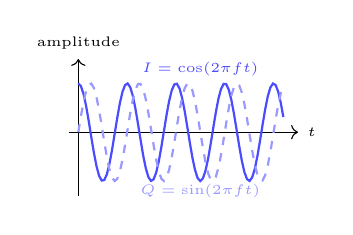
\begin{tikzpicture}[scale=0.62]
    \draw[->] (-0.2,0) -- (4.5,0) node[right, font=\tiny] {$t$};
    \draw[->] (0,-1.3) -- (0,1.5) node[above, font=\tiny] {amplitude};
    \draw[thick, blue!70, domain=0:4.2, samples=80]
      plot(\x, {cos(360*\x)});
    \draw[thick, blue!40, dashed, domain=0:4.2, samples=80]
      plot(\x, {sin(360*\x)});
    \node[font=\tiny, blue!70] at (2.5, 1.3) {$I = \cos(2\pi f t)$};
    \node[font=\tiny, blue!40] at (2.5, -1.2) {$Q = \sin(2\pi f t)$};
  \end{tikzpicture}\\
  \small
  $x(t) = I(t) + j\,Q(t)$\\
  Representa \textbf{fase e amplitude}\\
  Usado em: modulac\~{a}o, SDR, RF
  \end{block}
\end{column}
\begin{column}{0.48\textwidth}
  \begin{block}{\textcolor{orange!80}{Float} --- sinal real}
  \vspace{0.1cm}
  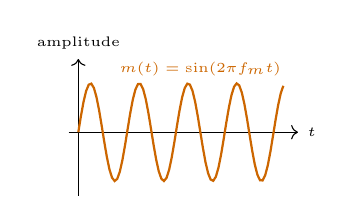
\begin{tikzpicture}[scale=0.62]
    \draw[->] (-0.2,0) -- (4.5,0) node[right, font=\tiny] {$t$};
    \draw[->] (0,-1.3) -- (0,1.5) node[above, font=\tiny] {amplitude};
    \draw[thick, orange!80!black, domain=0:4.2, samples=80]
      plot(\x, {sin(360*\x)});
    \node[font=\tiny, orange!80!black] at (2.5, 1.3) {$m(t) = \sin(2\pi f_m t)$};
  \end{tikzpicture}\\
  \small
  $m(t) \in \mathbb{R}$\\
  Sinal de \textbf{mensagem} (voz, m\'{u}sica)\\
  Usado em: \'{a}udio, banda-base, plots
  \end{block}
\end{column}
\end{columns}

\vspace{0.1cm}
\begin{center}
\small O bloco \texttt{Signal Source} pode gerar tanto \texttt{Complex} quanto \texttt{Float} --- altere o par\^{a}metro \textbf{Output Type}.
\end{center}
\end{frame}

% %%%%%%%%%%%%%%%%%%%%%%%%%%%%%%%%%%%%%%%%%%%%
\section{Bloco Throttle}
% %%%%%%%%%%%%%%%%%%%%%%%%%%%%%%%%%%%%%%%%%%%%

{
\setbeamercolor{background canvas}{bg=unbprimary}
\setbeamercolor{normal text}{fg=white}
\usebeamercolor[fg]{normal text}
\begin{frame}[plain,c]
\begin{center}
{\Huge\textbf{Bloco Throttle}}\\[0.8cm]
{\LARGE Controlando a velocidade da simulac\~{a}o}\\[0.5cm]
{\large Sem hardware, precisa de controle de taxa}
\end{center}
\end{frame}
}

\begin{frame}{Por que precisamos do Throttle?}
\textbf{Problema:} sem hardware real, blocos processam dados o \textbf{mais r\'{a}pido poss\'{\i}vel} $\rightarrow$ \alert{CPU a 100\%}!

\vspace{0.2cm}

\begin{center}
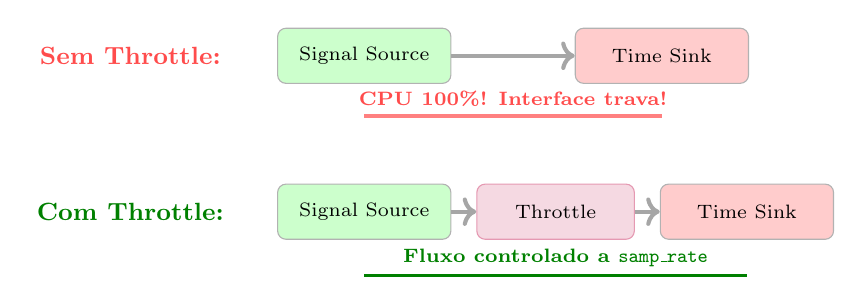
\begin{tikzpicture}[scale=0.9]
  % Sem Throttle
  \node[font=\small\bfseries, text=red!70] at (-2.5, 0) {Sem Throttle:};
  \node[grcsrc, minimum width=2.2cm] (s1) at (0.8,0) {Signal Source};
  \node[grcsink, minimum width=2.2cm] (k1) at (5.0,0) {Time Sink};
  \draw[grcarrow, line width=1.5pt] (s1) -- (k1);
  \node[font=\scriptsize, red!70] at (2.9, -0.6) {\textbf{CPU 100\%! Interface trava!}};
  \draw[very thick, red!50]
    (0.8,-0.85) -- (5.0,-0.85);

  % Com Throttle
  \node[font=\small\bfseries, text=cGreen] at (-2.5, -2.2) {Com Throttle:};
  \node[grcsrc, minimum width=2.2cm] (s2) at (0.8,-2.2) {Signal Source};
  \node[grcthrottle, minimum width=2.0cm] (t2) at (3.5,-2.2) {Throttle};
  \node[grcsink, minimum width=2.2cm] (k2) at (6.2,-2.2) {Time Sink};
  \draw[grcarrow, line width=1.5pt] (s2) -- (t2);
  \draw[grcarrow, line width=1.5pt] (t2) -- (k2);
  \node[font=\scriptsize, cGreen] at (3.5, -2.85) {\textbf{Fluxo controlado a \texttt{samp\_rate}}};
  \draw[very thick, cGreen] (0.8,-3.1) -- (6.2,-3.1);
\end{tikzpicture}
\end{center}

\vspace{0.1cm}

\begin{columns}
\begin{column}{0.55\textwidth}
  \begin{itemize}\setlength{\itemsep}{1pt}
    \item Limita amostras \`{a} taxa \texttt{samp\_rate}
    \item \alert{Usar apenas 1 Throttle por flowgraph}
  \end{itemize}
\end{column}
\begin{column}{0.42\textwidth}
  \begin{alertblock}{Quando n\~{a}o usar}
  \footnotesize Com hardware real (USRP, RTL-SDR, HackRF), o dispositivo controla a taxa.
  \end{alertblock}
\end{column}
\end{columns}
\end{frame}

\begin{frame}{Par\^{a}metros do Throttle}
\begin{columns}
\begin{column}{0.48\textwidth}
  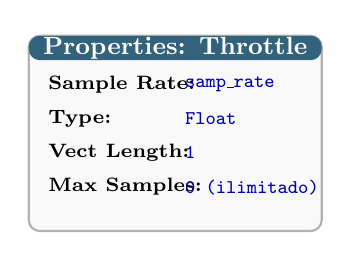
\begin{tikzpicture}[scale=0.62]
    \draw[rounded corners=4pt, thick, gray!60, fill=gray!5]
      (0,0.5) rectangle (6.0, 4.5);
    \fill[unbprimary!80, rounded corners=4pt] (0,4.0) -- (6.0,4.0) -- (6.0,4.5) -- (0,4.5) -- cycle;
    \node[text=white, font=\small\bfseries] at (3.0,4.25) {Properties: Throttle};
    \node[right, font=\scriptsize\bfseries] at (0.2, 3.5) {Sample Rate:};
    \node[right, font=\scriptsize\ttfamily, text=cBlue] at (3.0, 3.5) {samp\_rate};
    \node[right, font=\scriptsize\bfseries] at (0.2, 2.8) {Type:};
    \node[right, font=\scriptsize\ttfamily, text=cBlue] at (3.0, 2.8) {Float};
    \node[right, font=\scriptsize\bfseries] at (0.2, 2.1) {Vect Length:};
    \node[right, font=\scriptsize\ttfamily, text=cBlue] at (3.0, 2.1) {1};
    \node[right, font=\scriptsize\bfseries] at (0.2, 1.4) {Max Samples:};
    \node[right, font=\scriptsize\ttfamily, text=cBlue] at (3.0, 1.4) {0 (ilimitado)};
  \end{tikzpicture}
\end{column}
\begin{column}{0.48\textwidth}
  \textbf{Configurac\~{a}o t\'{\i}pica:}
  \begin{itemize}\setlength{\itemsep}{2pt}
    \item \textbf{Sample Rate}: usar \texttt{samp\_rate}
    \item \textbf{Type}: combinar com blocos conectados
    \item \textbf{Vect Length}: 1 (escalar)
  \end{itemize}

  \vspace{0.2cm}

  \begin{exampleblock}{Exemplo}
  \small Se \texttt{samp\_rate = 32000}: o Throttle limita a \textbf{32.000 amostras/s}.
  \end{exampleblock}
\end{column}
\end{columns}
\end{frame}

% %%%%%%%%%%%%%%%%%%%%%%%%%%%%%%%%%%%%%%%%%%%%
\section{Vari\'{a}veis}
% %%%%%%%%%%%%%%%%%%%%%%%%%%%%%%%%%%%%%%%%%%%%

{
\setbeamercolor{background canvas}{bg=unbprimary}
\setbeamercolor{normal text}{fg=white}
\usebeamercolor[fg]{normal text}
\begin{frame}[plain,c]
\begin{center}
{\Huge\textbf{Vari\'{a}veis}}\\[0.8cm]
{\LARGE Parametrizando o flowgraph}\\[0.5cm]
{\large Variable, QT GUI Range, QT GUI Chooser}
\end{center}
\end{frame}
}

\begin{frame}{Bloco Variable}
\begin{columns}
\begin{column}{0.50\textwidth}
  \textbf{O que \'{e}?}
  \begin{itemize}
    \item Define um \textbf{par\^{a}metro reutiliz\'{a}vel}
    \item Pode ser referenciado em qualquer bloco pelo nome
    \item Alterac\~{a}o em um \'{u}nico lugar atualiza \textbf{todos os blocos}
  \end{itemize}

  \vspace{0.2cm}

  \textbf{Vari\'{a}vel padr\~{a}o:} \texttt{samp\_rate}
  \begin{itemize}
    \item Criada automaticamente em todo novo flowgraph
    \item Valor padr\~{a}o: \texttt{32000} (32 kHz)
    \item Usada no Throttle e nos sinks
  \end{itemize}
\end{column}
\begin{column}{0.47\textwidth}
  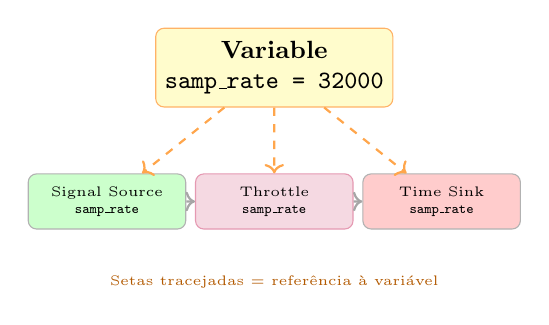
\begin{tikzpicture}[scale=0.85]
    % Bloco Variable
    \node[grcvar, minimum width=3cm, minimum height=1cm, font=\small] (var) at (3, 4.0)
      {\textbf{Variable}\\\texttt{samp\_rate = 32000}};
    % Blocos que usam
    \node[grcsrc, font=\tiny] (src) at (0.5, 2.0) {Signal Source\\\tiny\texttt{samp\_rate}};
    \node[grcthrottle, font=\tiny] (thr) at (3.0, 2.0) {Throttle\\\tiny\texttt{samp\_rate}};
    \node[grcsink, font=\tiny] (snk) at (5.5, 2.0) {Time Sink\\\tiny\texttt{samp\_rate}};
    % Setas de referência
    \draw[->, dashed, orange!70, thick] (var) -- (src);
    \draw[->, dashed, orange!70, thick] (var) -- (thr);
    \draw[->, dashed, orange!70, thick] (var) -- (snk);
    % Fluxo de dados
    \draw[grcarrow] (src) -- (thr);
    \draw[grcarrow] (thr) -- (snk);
    % Legenda
    \node[font=\tiny, text=orange!70!black] at (3.0, 0.8)
      {Setas tracejadas = refer\^{e}ncia \`{a} vari\'{a}vel};
  \end{tikzpicture}
\end{column}
\end{columns}
\end{frame}

\begin{frame}{Criando vari\'{a}veis personalizadas}
\begin{columns}
\begin{column}{0.48\textwidth}
  \small
  \begin{tabular}{lll}
    \hline
    \textbf{Nome} & \textbf{Valor} & \textbf{Uso} \\
    \hline
    \texttt{samp\_rate} & \texttt{32000} & Taxa de amostragem \\
    \texttt{freq}       & \texttt{1000}  & Freq. do sinal (Hz) \\
    \texttt{amp}        & \texttt{1.0}   & Amplitude \\
    \texttt{fc}         & \texttt{10000} & Freq. da portadora \\
    \hline
  \end{tabular}

  \vspace{0.2cm}

  \textbf{Express\~{o}es Python v\'{a}lidas:}
  \begin{itemize}\setlength{\itemsep}{1pt}
    \item \texttt{2 * 3.14159 * freq}
    \item \texttt{samp\_rate / 2}
    \item \texttt{int(samp\_rate * 0.1)}
  \end{itemize}
\end{column}
\begin{column}{0.48\textwidth}
  \begin{alertblock}{Express\~{o}es Python}
  \small Valores podem ser express\~{o}es Python:
  \begin{itemize}\setlength{\itemsep}{1pt}
    \item Operac\~{o}es matem\'{a}ticas
    \item Refer\^{e}ncias a outras vari\'{a}veis
    \item Fun\c{c}\~{o}es: \texttt{int()}, \texttt{round()}
    \item M\'{o}dulos: \texttt{import numpy as np}
  \end{itemize}
  \end{alertblock}

  \vspace{0.1cm}

  \begin{exampleblock}{Boas pr\'{a}ticas}
  \small
  \begin{itemize}\setlength{\itemsep}{1pt}
    \item Nomes \textbf{descritivos}: \texttt{freq\_msg}, n\~{a}o \texttt{f}
    \item Evite n\'{u}meros ``m\'{a}gicos'' nos blocos
  \end{itemize}
  \end{exampleblock}
\end{column}
\end{columns}
\end{frame}

\begin{frame}{Controles interativos: QT GUI Range}
\begin{columns}
\begin{column}{0.50\textwidth}
  \textbf{O bloco \texttt{QT GUI Range}:}
  \begin{itemize}\setlength{\itemsep}{1pt}
    \item Substitui o bloco \texttt{Variable}
    \item Cria um \textbf{slider} na interface gr\'{a}fica
    \item Permite alterar o valor \textbf{em tempo real}
  \end{itemize}

  \vspace{0.15cm}

  \textbf{Par\^{a}metros:}
  \begin{itemize}\setlength{\itemsep}{1pt}
    \item \textbf{ID}: nome da vari\'{a}vel (ex: \texttt{freq})
    \item \textbf{Default}: valor inicial
    \item \textbf{Start / Stop}: faixa do slider
    \item \textbf{Step}: incremento m\'{\i}nimo
  \end{itemize}
\end{column}
\begin{column}{0.47\textwidth}
  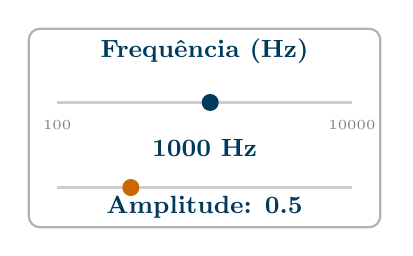
\begin{tikzpicture}[scale=0.72]
    \draw[rounded corners=4pt, thick, gray!60, fill=white]
      (0,0) rectangle (6.2, 3.5);
    \node[font=\small\bfseries, text=unbprimary] at (3.1, 3.1) {Frequ\^{e}ncia (Hz)};
    \draw[thick, gray!40] (0.5, 2.2) -- (5.7, 2.2);
    \fill[unbprimary] (3.2, 2.2) circle (0.15);
    \node[font=\tiny, gray] at (0.5, 1.8) {100};
    \node[font=\tiny, gray] at (5.7, 1.8) {10000};
    \node[font=\small\bfseries, text=unbprimary] at (3.1, 1.4) {1000 Hz};
    \draw[thick, gray!40] (0.5, 0.7) -- (5.7, 0.7);
    \fill[cOrange] (1.8, 0.7) circle (0.15);
    \node[font=\small\bfseries, text=unbprimary] at (3.1, 0.35) {Amplitude: 0.5};
  \end{tikzpicture}

  \vspace{0.15cm}

  \small Variar frequ\^{e}ncia, amplitude, ganho --- e ver o efeito \textbf{instantaneamente} nos gr\'{a}ficos!
\end{column}
\end{columns}
\end{frame}

% %%%%%%%%%%%%%%%%%%%%%%%%%%%%%%%%%%%%%%%%%%%%
\section{Blocos de Visualizac\~{a}o (Plots)}
% %%%%%%%%%%%%%%%%%%%%%%%%%%%%%%%%%%%%%%%%%%%%

{
\setbeamercolor{background canvas}{bg=unbprimary}
\setbeamercolor{normal text}{fg=white}
\usebeamercolor[fg]{normal text}
\begin{frame}[plain,c]
\begin{center}
{\Huge\textbf{Blocos de Visualizac\~{a}o}}\\[0.8cm]
{\LARGE Plots no dom\'{\i}nio do tempo e da frequ\^{e}ncia}\\[0.5cm]
{\large Time Sink, Frequency Sink, Waterfall, Constellation}
\end{center}
\end{frame}
}

\begin{frame}{QT GUI Time Sink --- dom\'{\i}nio do tempo}
\begin{columns}
\begin{column}{0.48\textwidth}
  \textbf{Visualiza a forma de onda} $x(t)$ vs $t$

  \vspace{0.1cm}

  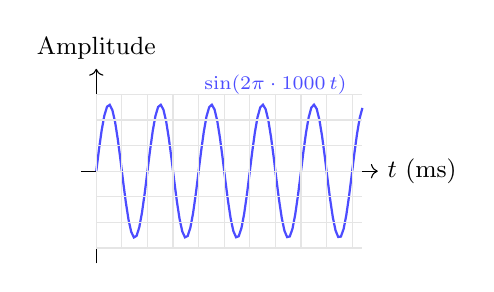
\begin{tikzpicture}[scale=0.65]
    \draw[->] (-0.3,0) -- (5.5,0) node[right, font=\small] {$t$ (ms)};
    \draw[->] (0,-1.8) -- (0,2.0) node[above, font=\small] {Amplitude};
    \draw[thick, blue!70, domain=0:5.2, samples=100]
      plot(\x, {1.3*sin(360*\x)});
    \draw[gray!20] (0,-1.5) grid[step=0.5] (5.2,1.5);
    \node[font=\scriptsize, blue!70] at (3.5, 1.7) {$\sin(2\pi \cdot 1000\, t)$};
  \end{tikzpicture}

  \vspace{0.1cm}

  \textbf{Par\^{a}metros principais:}
  \begin{itemize}\setlength{\itemsep}{1pt}
    \item \textbf{Number of Points}: amostras exibidas
    \item \textbf{Sample Rate}: \texttt{samp\_rate}
    \item \textbf{Autoscale}: ajuste autom\'{a}tico de eixo Y
  \end{itemize}
\end{column}
\begin{column}{0.48\textwidth}
  \textbf{M\'{u}ltiplos sinais:}

  \vspace{0.1cm}

  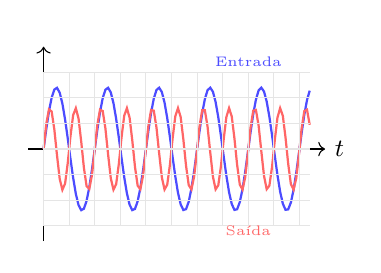
\begin{tikzpicture}[scale=0.65]
    \draw[->] (-0.3,0) -- (5.5,0) node[right, font=\small] {$t$};
    \draw[->] (0,-1.8) -- (0,2.0) node[above, font=\small] {};
    \draw[thick, blue!70, domain=0:5.2, samples=100]
      plot(\x, {1.2*sin(360*\x)});
    \draw[thick, red!60, domain=0:5.2, samples=100]
      plot(\x, {0.8*sin(720*\x)});
    \draw[gray!20] (0,-1.5) grid[step=0.5] (5.2,1.5);
    \node[font=\tiny, blue!70] at (4.0, 1.7) {Entrada};
    \node[font=\tiny, red!60] at (4.0, -1.6) {Sa\'{\i}da};
  \end{tikzpicture}

  \vspace{0.1cm}

  \begin{exampleblock}{M\'{u}ltiplas entradas}
  \small Conecte \textbf{v\'{a}rias entradas} no mesmo Time Sink para comparar sinais.
  Aumente \texttt{Number of Inputs}.
  \end{exampleblock}
\end{column}
\end{columns}
\end{frame}

\begin{frame}{QT GUI Frequency Sink --- dom\'{\i}nio da frequ\^{e}ncia}
\begin{columns}
\begin{column}{0.48\textwidth}
  \textbf{Visualiza o espectro} $|X(f)|$ em dB

  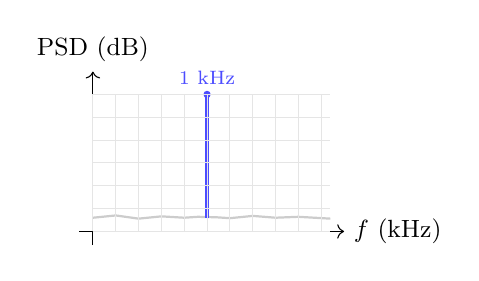
\begin{tikzpicture}[scale=0.58]
    \draw[->] (-0.3,0) -- (5.5,0) node[right, font=\small] {$f$ (kHz)};
    \draw[->] (0,-0.3) -- (0,3.5) node[above, font=\small] {PSD (dB)};
    \draw[thick, gray!40] (0,0.3) -- (0.5,0.35) -- (1.0,0.28) -- (1.5,0.33) -- (2.0,0.30) -- (2.3,0.32) -- (2.7,0.31) -- (3.0,0.29) -- (3.5,0.34) -- (4.0,0.30) -- (4.5,0.32) -- (5.2,0.28);
    \draw[very thick, blue!70] (2.5, 0.3) -- (2.5, 3.0);
    \fill[blue!70] (2.5, 3.0) circle (0.08);
    \node[font=\scriptsize, blue!70, above] at (2.5, 3.0) {1 kHz};
    \draw[gray!20] (0,0) grid[step=0.5] (5.2,3.0);
  \end{tikzpicture}

  \vspace{0.1cm}

  \textbf{Par\^{a}metros principais:}
  \begin{itemize}\setlength{\itemsep}{1pt}
    \item \textbf{FFT Size}: resoluc\~{a}o (1024, 2048, 4096)
    \item \textbf{Center Freq}: frequ\^{e}ncia central
    \item \textbf{Average}: suavizac\~{a}o do espectro
  \end{itemize}
\end{column}
\begin{column}{0.48\textwidth}
  \textbf{O que o Frequency Sink mostra:}
  \begin{itemize}\setlength{\itemsep}{1pt}
    \item Componentes de frequ\^{e}ncia do sinal
    \item Pot\^{e}ncia Espectral (PSD) em dB
    \item Harm\^{o}nicas, ru\'{\i}do de fundo
  \end{itemize}

  \vspace{0.15cm}

  \textbf{FFT Size --- resoluc\~{a}o:}
  \vspace{-0.2cm}
  \[\Delta f = \frac{f_s}{N_{\text{FFT}}}\]
  \vspace{-0.3cm}

  \begin{itemize}\setlength{\itemsep}{1pt}
    \item $f_s = 32000$, $N_{\text{FFT}} = 1024$
      $\Rightarrow \Delta f = 31{,}25$ Hz
    \item Mais pontos = melhor resoluc\~{a}o, por\'{e}m mais lento
  \end{itemize}
\end{column}
\end{columns}
\end{frame}

\begin{frame}{Outros blocos de visualizac\~{a}o}
\begin{columns}
\begin{column}{0.48\textwidth}
  \textbf{QT GUI Waterfall Sink}
  \begin{itemize}\setlength{\itemsep}{1pt}
    \item Espectrograma: frequ\^{e}ncia $\times$ tempo
    \item Cor indica a pot\^{e}ncia (dB)
    \item \'{O}timo para sinais que variam no tempo
  \end{itemize}

  \vspace{0.1cm}

  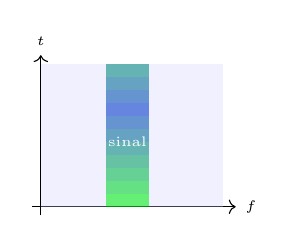
\begin{tikzpicture}[scale=0.55]
    \draw[->] (-0.2,0) -- (4.5,0) node[right, font=\tiny] {$f$};
    \draw[->] (0,-0.2) -- (0,3.5) node[above, font=\tiny] {$t$};
    \foreach \y/\c in {0/10,0.3/20,0.6/30,0.9/40,1.2/50,1.5/60,1.8/70,2.1/80,2.4/70,2.7/60,3.0/50} {
      \fill[blue!\c!green, opacity=0.6] (1.5,\y) rectangle (2.5,{\y+0.3});
      \fill[blue!20, opacity=0.3] (0,\y) rectangle (1.5,{\y+0.3});
      \fill[blue!20, opacity=0.3] (2.5,\y) rectangle (4.2,{\y+0.3});
    }
    \node[font=\tiny, text=white] at (2.0, 1.5) {sinal};
  \end{tikzpicture}

  \vspace{0.1cm}
  \small \textbf{Scope Sink}: oscilosc\'{o}pio virtual com trigger
\end{column}
\begin{column}{0.48\textwidth}
  \textbf{QT GUI Constellation Sink}
  \begin{itemize}\setlength{\itemsep}{1pt}
    \item Diagrama I/Q (parte real vs. imagin\'{a}ria)
    \item Usado em modulac\~{o}es digitais (QAM, PSK)
    \item Entrada: \textbf{Complex} obrigat\'{o}rio
  \end{itemize}

  \vspace{0.1cm}

  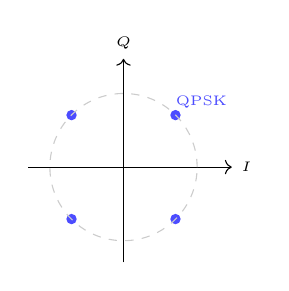
\begin{tikzpicture}[scale=0.55]
    \draw[->] (-2.2,0) -- (2.5,0) node[right, font=\tiny] {$I$};
    \draw[->] (0,-2.2) -- (0,2.5) node[above, font=\tiny] {$Q$};
    \fill[blue!70] (1.2, 1.2) circle (0.12);
    \fill[blue!70] (-1.2, 1.2) circle (0.12);
    \fill[blue!70] (-1.2, -1.2) circle (0.12);
    \fill[blue!70] (1.2, -1.2) circle (0.12);
    \node[font=\tiny, text=blue!70] at (1.8, 1.5) {QPSK};
    \draw[dashed, gray!40] (0,0) circle (1.7);
  \end{tikzpicture}
\end{column}
\end{columns}
\end{frame}

% %%%%%%%%%%%%%%%%%%%%%%%%%%%%%%%%%%%%%%%%%%%%
\section{Primeiro Flowgraph: Passo a Passo}
% %%%%%%%%%%%%%%%%%%%%%%%%%%%%%%%%%%%%%%%%%%%%

{
\setbeamercolor{background canvas}{bg=unbprimary}
\setbeamercolor{normal text}{fg=white}
\usebeamercolor[fg]{normal text}
\begin{frame}[plain,c]
\begin{center}
{\Huge\textbf{Primeiro Flowgraph}}\\[0.8cm]
{\LARGE Passo a passo no GRC}\\[0.5cm]
{\large Senoide + Throttle + Plots}
\end{center}
\end{frame}
}

\begin{frame}{Flowgraph 1: Senoide no tempo e na frequ\^{e}ncia}
\begin{center}
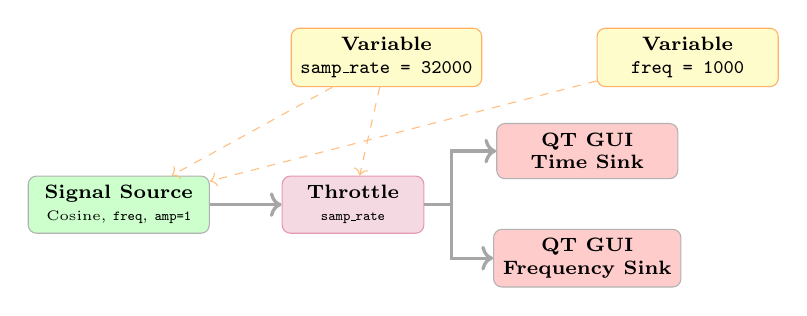
\begin{tikzpicture}[scale=0.85]
  \node[grcvar, minimum width=2.3cm] (var) at (4.0, 2.2)
    {\textbf{Variable}\\\texttt{samp\_rate = 32000}};
  \node[grcvar, minimum width=2.3cm] (vf) at (8.5, 2.2)
    {\textbf{Variable}\\\texttt{freq = 1000}};
  \node[grcsrc, minimum width=2.3cm] (src) at (0, 0)
    {\textbf{Signal Source}\\\tiny Cosine, \texttt{freq}, \texttt{amp=1}};
  \node[grcthrottle, minimum width=1.8cm] (thr) at (3.5, 0)
    {\textbf{Throttle}\\\tiny \texttt{samp\_rate}};
  \node[grcsink, minimum width=2.3cm] (time) at (7.0, 0.8)
    {\textbf{QT GUI}\\\textbf{Time Sink}};
  \node[grcsink, minimum width=2.3cm] (freq) at (7.0, -0.8)
    {\textbf{QT GUI}\\\textbf{Frequency Sink}};
  \draw[grcarrow, line width=1.2pt] (src) -- (thr);
  \draw[grcarrow, line width=1.2pt] (thr.east) -- ++(0.4,0) |- (time);
  \draw[grcarrow, line width=1.2pt] (thr.east) -- ++(0.4,0) |- (freq);
  \draw[->, dashed, orange!50, thin] (var) -- (src);
  \draw[->, dashed, orange!50, thin] (var) -- (thr);
  \draw[->, dashed, orange!50, thin] (vf) -- (src);
\end{tikzpicture}
\end{center}
\end{frame}

\begin{frame}{Flowgraph 1: Passo a passo}
\begin{enumerate}
  \item Abra o GRC $\rightarrow$ novo flowgraph (j\'{a} vem com \texttt{samp\_rate} e \texttt{Options})
  \item Adicione: \texttt{Signal Source} $\rightarrow$ \texttt{Throttle} $\rightarrow$ \texttt{QT GUI Time Sink}
  \item Adicione um \texttt{QT GUI Frequency Sink} conectado ap\'{o}s o Throttle
  \item Crie a vari\'{a}vel \texttt{freq = 1000} e use-a no Signal Source
  \item \alert{Execute} (F6) e observe os plots!
\end{enumerate}

\vspace{0.3cm}

\begin{exampleblock}{Arquivo pronto}
\texttt{exemplo\_01\_senoide.grc} --- abra no GRC e execute com F6
\end{exampleblock}
\end{frame}

\begin{frame}{Configurac\~{a}o do Signal Source --- par\^{a}metros}
\begin{columns}
\begin{column}{0.50\textwidth}
  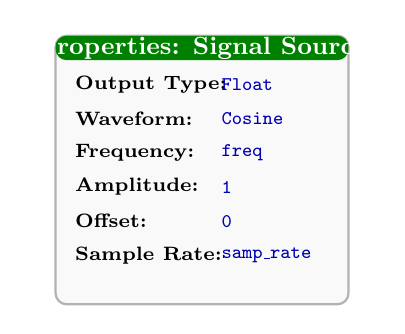
\begin{tikzpicture}[scale=0.62]
    \draw[rounded corners=4pt, thick, gray!60, fill=gray!5]
      (0,0) rectangle (6.0, 5.5);
    \fill[cGreen, rounded corners=4pt] (0,5.0) -- (6.0,5.0) -- (6.0,5.5) -- (0,5.5) -- cycle;
    \node[text=white, font=\small\bfseries] at (3.0,5.25) {Properties: Signal Source};
    \node[right, font=\scriptsize\bfseries] at (0.2, 4.5) {Output Type:};
    \node[right, font=\scriptsize\ttfamily, text=cBlue] at (3.2, 4.5) {Float};
    \node[right, font=\scriptsize\bfseries] at (0.2, 3.8) {Waveform:};
    \node[right, font=\scriptsize\ttfamily, text=cBlue] at (3.2, 3.8) {Cosine};
    \node[right, font=\scriptsize\bfseries] at (0.2, 3.1) {Frequency:};
    \node[right, font=\scriptsize\ttfamily, text=cBlue] at (3.2, 3.1) {freq};
    \node[right, font=\scriptsize\bfseries] at (0.2, 2.4) {Amplitude:};
    \node[right, font=\scriptsize\ttfamily, text=cBlue] at (3.2, 2.4) {1};
    \node[right, font=\scriptsize\bfseries] at (0.2, 1.7) {Offset:};
    \node[right, font=\scriptsize\ttfamily, text=cBlue] at (3.2, 1.7) {0};
    \node[right, font=\scriptsize\bfseries] at (0.2, 1.0) {Sample Rate:};
    \node[right, font=\scriptsize\ttfamily, text=cBlue] at (3.2, 1.0) {samp\_rate};
  \end{tikzpicture}
\end{column}
\begin{column}{0.47\textwidth}
  \textbf{Campos importantes:}
  \begin{itemize}\setlength{\itemsep}{2pt}
    \item \textbf{Output Type}: \texttt{Float} ou \texttt{Complex}
    \item \textbf{Waveform}: forma de onda
    \item \textbf{Frequency}: usar vari\'{a}vel \texttt{freq}
    \item \textbf{Sample Rate}: usar \texttt{samp\_rate}
  \end{itemize}

  \vspace{0.15cm}

  \small Para sinal anal\'{\i}tico $e^{j2\pi ft}$,\\
  altere Output Type para \texttt{Complex}.
\end{column}
\end{columns}
\end{frame}

\begin{frame}{Configurac\~{a}o do Signal Source --- formas de onda}
\begin{center}
  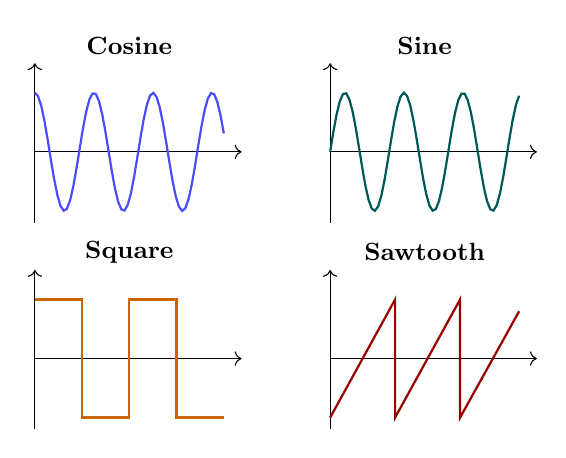
\begin{tikzpicture}[scale=0.75]
    % Cosine
    \draw[->] (0,0) -- (3.5,0); \draw[->] (0,-1.2) -- (0,1.5);
    \draw[thick, blue!70, domain=0:3.2, samples=60] plot(\x, {cos(360*\x)});
    \node[font=\small\bfseries] at (1.6, 1.8) {Cosine};
    % Sine
    \begin{scope}[xshift=5cm]
    \draw[->] (0,0) -- (3.5,0); \draw[->] (0,-1.2) -- (0,1.5);
    \draw[thick, cTeal, domain=0:3.2, samples=60] plot(\x, {sin(360*\x)});
    \node[font=\small\bfseries] at (1.6, 1.8) {Sine};
    \end{scope}
    % Square
    \begin{scope}[yshift=-3.5cm]
    \draw[->] (0,0) -- (3.5,0); \draw[->] (0,-1.2) -- (0,1.5);
    \draw[thick, cOrange] (0,1) -- (0.8,1) -- (0.8,-1) -- (1.6,-1) -- (1.6,1) -- (2.4,1) -- (2.4,-1) -- (3.2,-1);
    \node[font=\small\bfseries] at (1.6, 1.8) {Square};
    \end{scope}
    % Sawtooth
    \begin{scope}[xshift=5cm, yshift=-3.5cm]
    \draw[->] (0,0) -- (3.5,0); \draw[->] (0,-1.2) -- (0,1.5);
    \draw[thick, cRed] (0,-1) -- (1.1,1) -- (1.1,-1) -- (2.2,1) -- (2.2,-1) -- (3.2,0.8);
    \node[font=\small\bfseries] at (1.6, 1.8) {Sawtooth};
    \end{scope}
  \end{tikzpicture}
\end{center}
\end{frame}

\begin{frame}{Flowgraph 2: Controle interativo com slider}
\begin{center}
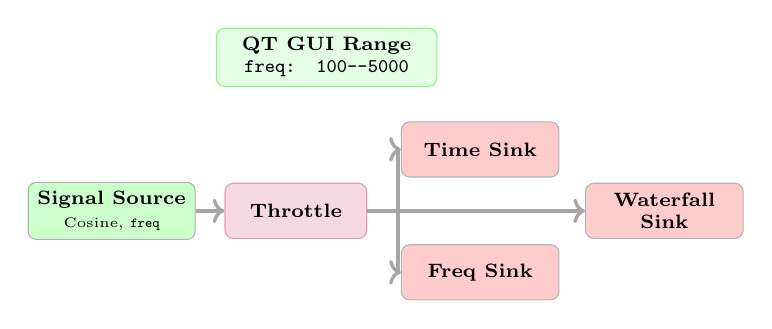
\begin{tikzpicture}[scale=0.78]
  % QT GUI Range
  \node[grcvar, minimum width=2.8cm, fill=green!10, draw=green!50] (slider) at (3.5, 2.5)
    {\textbf{QT GUI Range}\\\texttt{freq: 100--5000}};

  % Blocos
  \node[grcsrc, minimum width=2.0cm] (src) at (0, 0)
    {\textbf{Signal Source}\\\tiny Cosine, \texttt{freq}};
  \node[grcthrottle, minimum width=1.8cm] (thr) at (3.0, 0)
    {\textbf{Throttle}};
  \node[grcsink, minimum width=2.0cm] (time) at (6.0, 1.0)
    {\textbf{Time Sink}};
  \node[grcsink, minimum width=2.0cm] (fft) at (6.0, -1.0)
    {\textbf{Freq Sink}};
  \node[grcsink, minimum width=2.0cm] (wf) at (9.0, 0)
    {\textbf{Waterfall}\\\textbf{Sink}};

  % Conexões
  \draw[grcarrow, line width=1.2pt] (src) -- (thr);
  \draw[grcarrow, line width=1.2pt] (thr.east) -- ++(0.5,0) |- (time);
  \draw[grcarrow, line width=1.2pt] (thr.east) -- ++(0.5,0) |- (fft);
  \draw[grcarrow, line width=1.2pt] (thr.east) -- ++(0.5,0) |- (wf);
\end{tikzpicture}
\end{center}

\vspace{0.1cm}

\textbf{Exerc\'{\i}cio:}
\begin{enumerate}
  \item Substitua o bloco \texttt{Variable} (\texttt{freq}) por um \texttt{QT GUI Range}
  \item Configure: \texttt{Start=100}, \texttt{Stop=5000}, \texttt{Step=100}, \texttt{Default=1000}
  \item Adicione um \texttt{QT GUI Waterfall Sink}
  \item Execute e \textbf{mova o slider} --- observe a frequ\^{e}ncia mudar nos 3 plots!
\end{enumerate}
\end{frame}

\begin{frame}{Flowgraph 3: Somando dois sinais}
\begin{center}
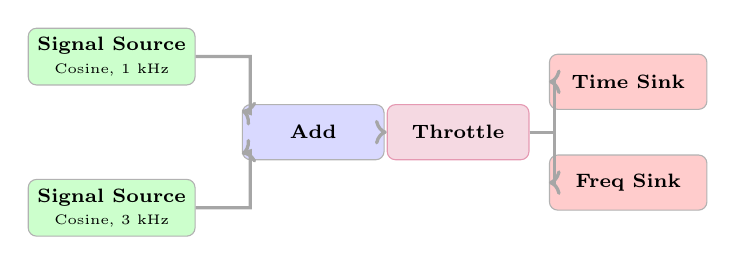
\begin{tikzpicture}[scale=0.8]
  \node[grcsrc, minimum width=2.0cm] (s1) at (0, 1.2)
    {\textbf{Signal Source}\\\tiny Cosine, 1 kHz};
  \node[grcsrc, minimum width=2.0cm] (s2) at (0, -1.2)
    {\textbf{Signal Source}\\\tiny Cosine, 3 kHz};
  \node[grcproc, minimum width=1.8cm] (add) at (3.2, 0)
    {\textbf{Add}};
  \node[grcthrottle, minimum width=1.8cm] (thr) at (5.5, 0)
    {\textbf{Throttle}};
  \node[grcsink, minimum width=2.0cm] (time) at (8.2, 0.8)
    {\textbf{Time Sink}};
  \node[grcsink, minimum width=2.0cm] (fft) at (8.2, -0.8)
    {\textbf{Freq Sink}};
  \draw[grcarrow, line width=1.2pt] (s1) -| (2.2, 0.3) -- (add);
  \draw[grcarrow, line width=1.2pt] (s2) -| (2.2, -0.3) -- (add);
  \draw[grcarrow, line width=1.2pt] (add) -- (thr);
  \draw[grcarrow, line width=1.2pt] (thr.east) -- ++(0.4,0) |- (time);
  \draw[grcarrow, line width=1.2pt] (thr.east) -- ++(0.4,0) |- (fft);
\end{tikzpicture}
\end{center}

\begin{columns}
\begin{column}{0.48\textwidth}
  \textbf{O que observar:}
  \begin{itemize}\setlength{\itemsep}{1pt}
    \item \textbf{Time Sink}: forma de onda composta
    \item \textbf{Freq Sink}: dois picos em 1 kHz e 3 kHz
  \end{itemize}
  \vspace{0.1cm}
  $x(t) = \cos(2\pi \cdot 1000\,t) + \cos(2\pi \cdot 3000\,t)$
\end{column}
\begin{column}{0.48\textwidth}
  \textbf{Desafio:}
  \begin{itemize}\setlength{\itemsep}{1pt}
    \item Adicione um \textbf{terceiro} sinal em 5 kHz
    \item Observe 3 picos no espectro
    \item Use \texttt{QT GUI Range} para variar amplitudes
  \end{itemize}
\end{column}
\end{columns}
\end{frame}

% %%%%%%%%%%%%%%%%%%%%%%%%%%%%%%%%%%%%%%%%%%%%
\section{Resumo e Pr\'{o}ximos Passos}
% %%%%%%%%%%%%%%%%%%%%%%%%%%%%%%%%%%%%%%%%%%%%

{
\setbeamercolor{background canvas}{bg=unbprimary}
\setbeamercolor{normal text}{fg=white}
\usebeamercolor[fg]{normal text}
\begin{frame}[plain,c]
\begin{center}
{\Huge\textbf{Resumo}}\\[0.8cm]
{\LARGE O que aprendemos hoje}
\end{center}
\end{frame}
}

\begin{frame}{Resumo da aula}
\begin{columns}
\begin{column}{0.48\textwidth}
  \begin{block}{Conceitos aprendidos}
  \begin{enumerate}\setlength{\itemsep}{2pt}
    \item \textbf{Flowgraph}: Source $\to$ Processing $\to$ Sink
    \item \textbf{Tipos de dados}: Complex, Float, Int, Short, Byte
    \item \textbf{Throttle}: controla taxa de simulac\~{a}o
    \item \textbf{Vari\'{a}veis}: parametrizam o flowgraph
    \item \textbf{QT GUI Range}: controle interativo
    \item \textbf{Plots}: Time, Freq, Waterfall, Constellation
  \end{enumerate}
  \end{block}
\end{column}
\begin{column}{0.48\textwidth}
  \begin{exampleblock}{Atalhos \'{u}teis do GRC}
  \small
  \begin{tabular}{ll}
    \textbf{F5} & Gerar flowgraph \\
    \textbf{F6} & Executar \\
    \textbf{F7} & Parar execuc\~{a}o \\
    \textbf{D}  & Desabilitar bloco \\
    \textbf{E}  & Habilitar bloco \\
    \textbf{R}  & Rotacionar bloco \\
    \textbf{Ctrl+F} & Buscar blocos \\
  \end{tabular}
  \end{exampleblock}
\end{column}
\end{columns}
\end{frame}

\begin{frame}{Exemplos e pr\'{o}ximos passos}
\begin{columns}
\begin{column}{0.48\textwidth}
  \begin{exampleblock}{Exemplos dispon\'{\i}veis}
  Abra no GRC e execute com F6:

  \vspace{0.2cm}

  \texttt{exemplo\_01\_senoide.grc}\\
  {\small Senoide + Time Sink + Freq Sink}

  \vspace{0.15cm}

  \texttt{exemplo\_02\_slider.grc}\\
  {\small Sliders interativos + Waterfall}

  \vspace{0.15cm}

  \texttt{exemplo\_03\_soma\_sinais.grc}\\
  {\small Soma de 1 kHz + 3 kHz}
  \end{exampleblock}
\end{column}
\begin{column}{0.48\textwidth}
  \begin{alertblock}{Pr\'{o}xima aula}
  \textbf{Pr\'{a}tica 1:} An\'{a}lise Espectral (FFT)

  \vspace{0.2cm}

  Aplicac\~{a}o dos conceitos de Fourier no GNU Radio
  \end{alertblock}
\end{column}
\end{columns}
\end{frame}

% ============================================
% ENCERRAMENTO
% ============================================
\begin{frame}{D\'{u}vidas?}
\begin{center}
\Large \textbf{Laborat\'{o}rio PRICOM --- GNU Radio}\\
\large Introduc\~{a}o ao GNU Radio Companion
\vspace{0.8cm}

\normalsize
\textbf{Prof.} \autorNome\\
\href{mailto:\autorEmail}{\autorEmail}
\vspace{0.4cm}

\textbf{\laboratorioFinal}\\
\universidadeFinal
\vspace{0.5cm}

\large \alert{Abra o GRC e experimente!}
\end{center}
\end{frame}

\end{document}
